\chapter{Aesthetic specifications}\label{cha:specifications}

This appendix summarises the various formats that \textbf{grid} drawing
functions take. Most of this information is available scattered
throughout the R documentation. This appendix brings it all together in
one place. \index{Aesthetics!specifications}

\section{Colour}\label{sec:colourux5fspec}

Colours can be specified with: \index{Colour!specifying}

\begin{itemize}
\itemsep1pt\parskip0pt\parsep0pt
\item
  A \textbf{name}, e.g., \texttt{"red"}. The colours are displayed in
  Figure\textasciitilde{}\ref{fig:colours}, and can be listed in more
  detail with \texttt{colours()}. The Stowers Institute provides a nice
  printable pdf that lists all colours:
  \url{http://research.stowers-institute.org/efg/R/Color/Chart/}.
\item
  An \textbf{rgb specification}, with a string of the form
  \texttt{"\#RRGGBB"} where each of the pairs \texttt{RR\},}GG\},
  \texttt{BB\} consists of two hexadecimal digits giving a value in the range}00\}
  to
  \texttt{FF\}.  Partially transparent can be made with \textbackslash{}f\{alpha\}, e.g.,}alpha(``red'',
  0.5)\}.
\item
  An \textbf{NA}, for a completely transparent colour.
\end{itemize}

The functions \texttt{rgb()}, \texttt{hsv()}, \texttt{hcl()} can be used
to create colours specified in different colour spaces.

\section{Line type}\label{sec:line-type-spec}

Line types can be specified with: \index{Line type!specifying}

\begin{itemize}
\itemsep1pt\parskip0pt\parsep0pt
\item
  An \textbf{integer} or \textbf{name}: 0=blank, 1=solid, 2=dashed,
  3=dotted, 4=dotdash, 5=longdash, 6=twodash), illustrated in
  Figure\textasciitilde{}\ref{fig:linetype}. *b The lengths of on/off
  stretches of line. This is done with a string of an even number (up to
  eight) of hexadecimal digits which give the lengths in consecutive
  positions in the string. For example, the string \texttt{"33"}
  specifies three units on followed by three off and \texttt{"3313"}
  specifies three units on followed by three off followed by one on and
  finally three off.
\end{itemize}

The five standard dash-dot line types described above correspond to 44,
13, 134, 73 and 2262.

Note that \texttt{NA} is not a valid value for \texttt{lty}.

\section{Shape}\label{sec:shape-spec}

Shapes take four types of values: \index{Shape!specifying}

\begin{itemize}
\itemsep1pt\parskip0pt\parsep0pt
\item
  An \textbf{integer} in $[0, 25]$, illustrated in
  Figure\textasciitilde{}\ref{fig:shape}.
\item
  A \textbf{single character}, to use that character as a plotting
  symbol.\\
\item
  A \texttt{.} to draw the smallest rectangle that is visible (i.e.,
  about one pixel).
\item
  An \texttt{NA}, to draw nothing.
\end{itemize}

While all symbols have a foreground colour, symbols 19--25 also take a
background colour (fill).

\section{Size}\label{sec:size}

Throughout \texttt{ggplot}, for text height, point size and line width,
size is specified in millimetres. \index{Size!specifying}

\section{Justification}\label{sec:justification-spec}

Justification of a string (or legend) defines the location within the
string that is placed at the given position. There are two values for
horizontal and vertical justification. The values can be:
\index{Text justification} \indexc{hjust} \indexc{vjust}

\begin{itemize}
\itemsep1pt\parskip0pt\parsep0pt
\item
  A \textbf{string}: \texttt{"left"}, \texttt{"right"},
  \texttt{"centre"}, \texttt{"center"}, \texttt{"bottom"}, and
  \texttt{"top"}.
\item
  A \textbf{number} between 0 and 1, giving the position within the
  string (from bottom-left corner). These values are demonstrated in
  Figure\textasciitilde{}\ref{fig:justification}.
\end{itemize}

\begin{figure}[htbp]
  \centering
  \subfigure[All named colours in Luv space]{
    \label{fig:colours}
    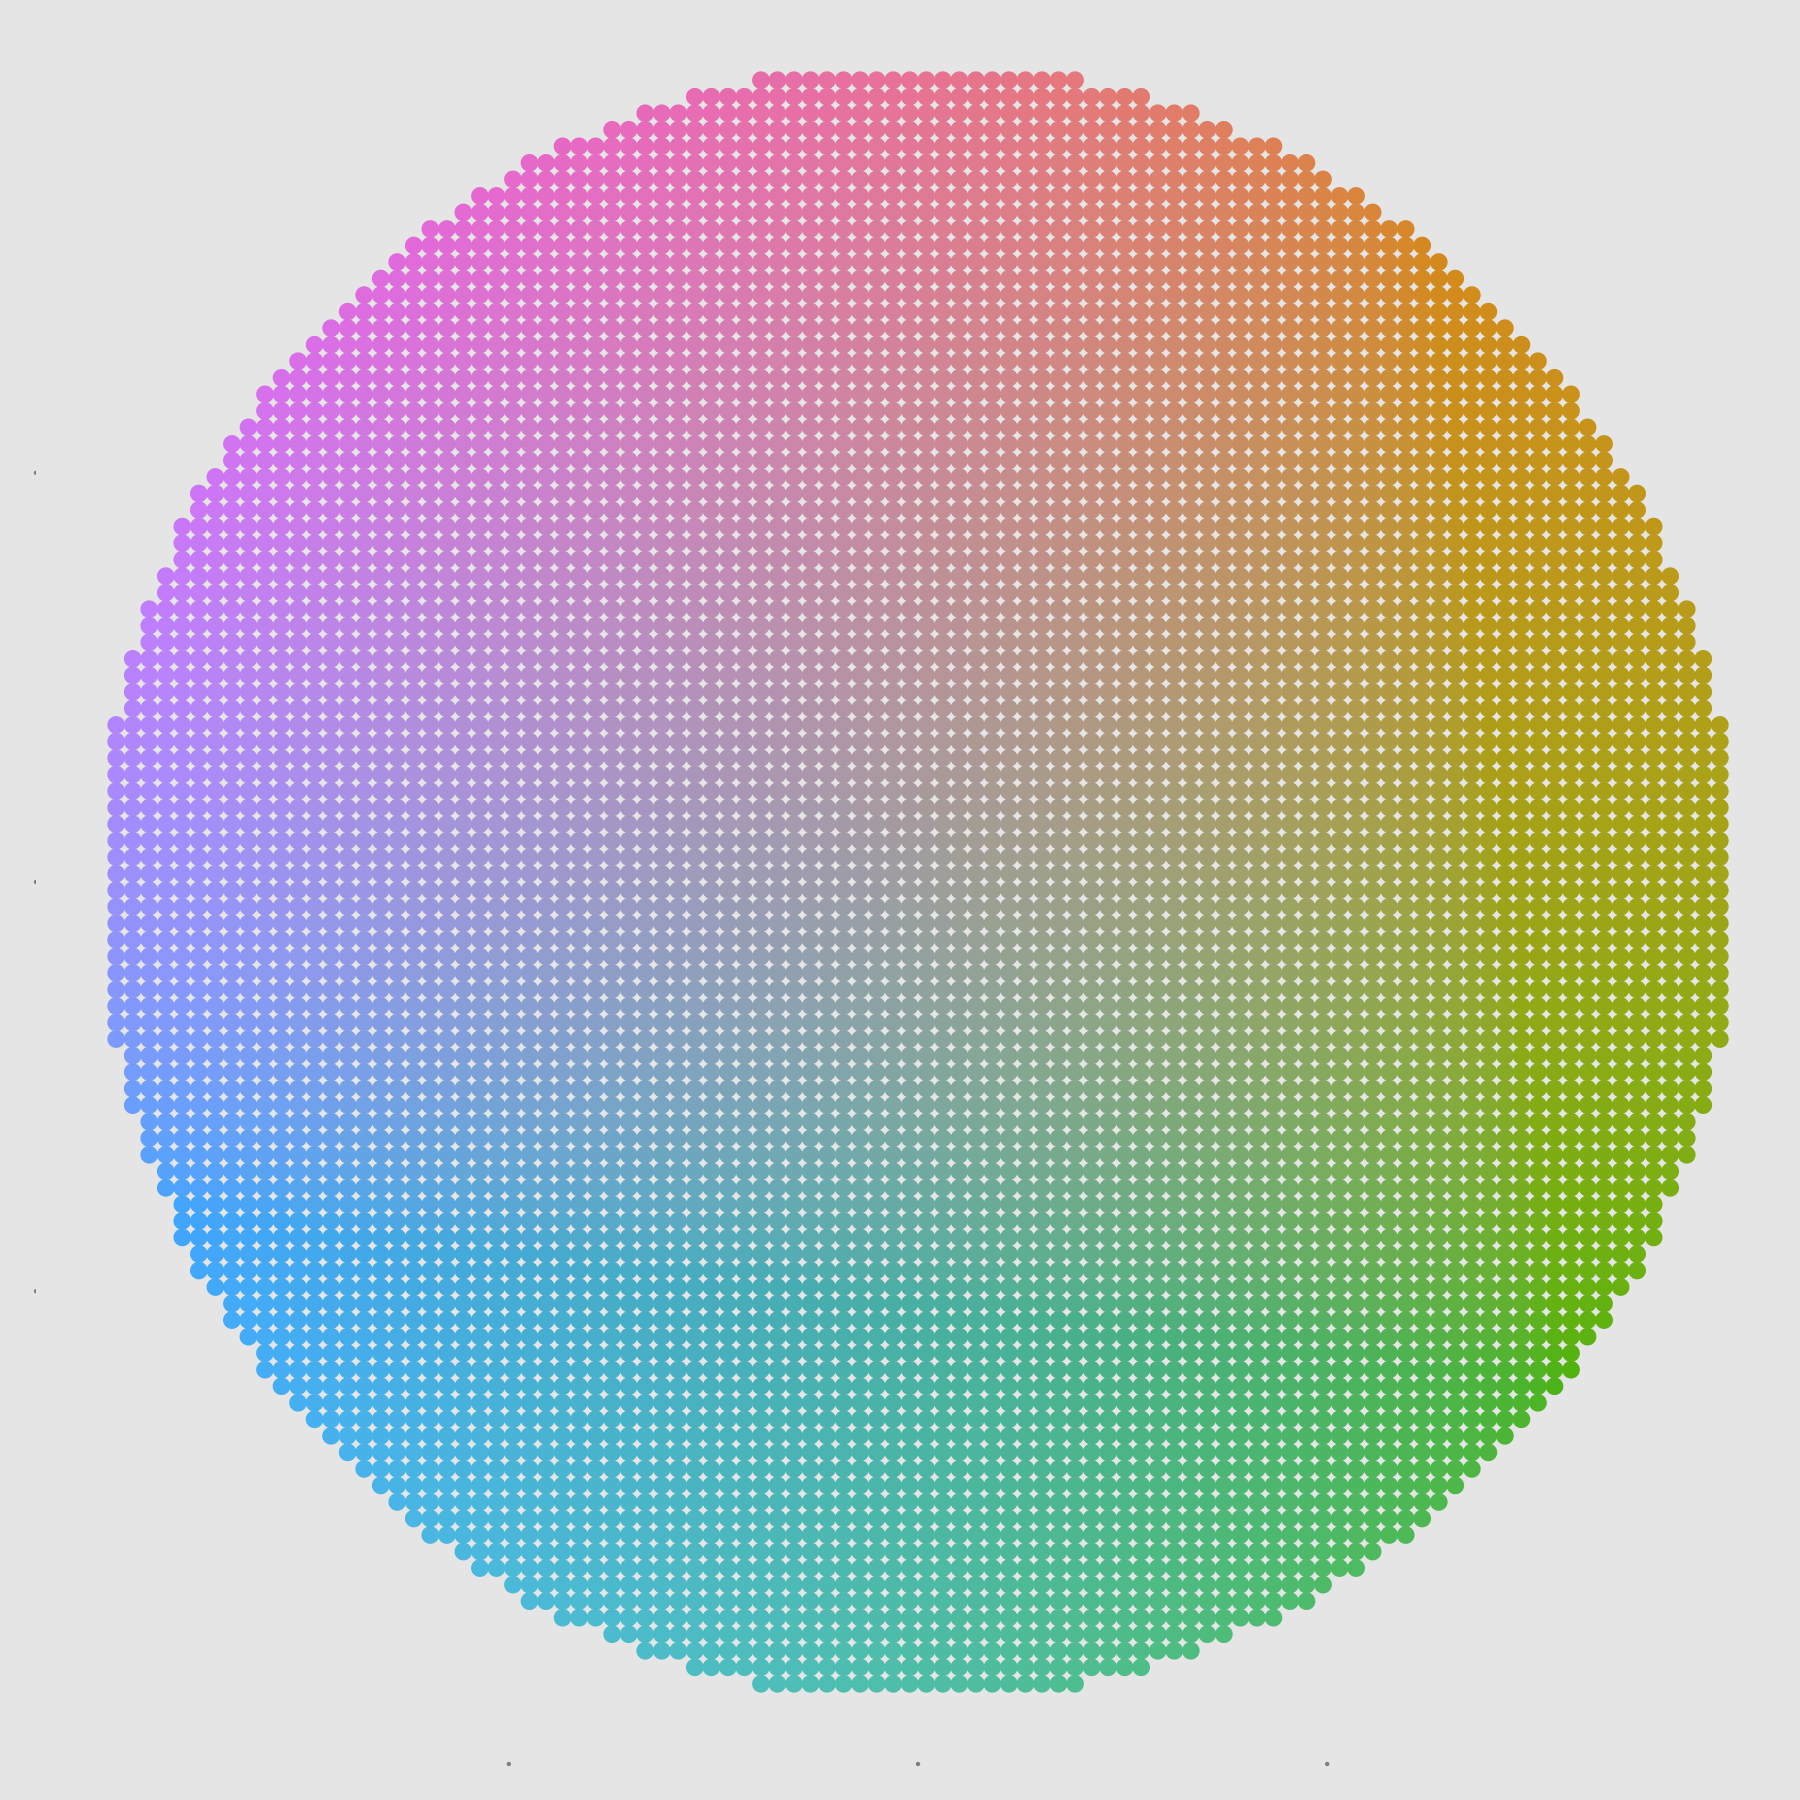
\includegraphics[width=0.45\linewidth]{diagrams/spec-colour}
  }
  \subfigure[Built-in line types]{
    \label{fig:linetype}
    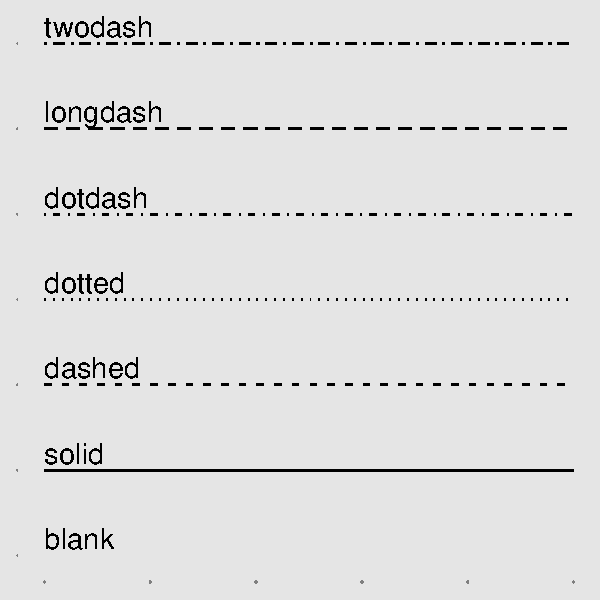
\includegraphics[width=0.45\linewidth]{diagrams/spec-linetype}
  }
  \subfigure[R plotting symbols.  Colour is black, and fill is blue.  Symbol 25 (not shown) is symbol 24 rotated 180 degrees.]{
    \label{fig:shape}
    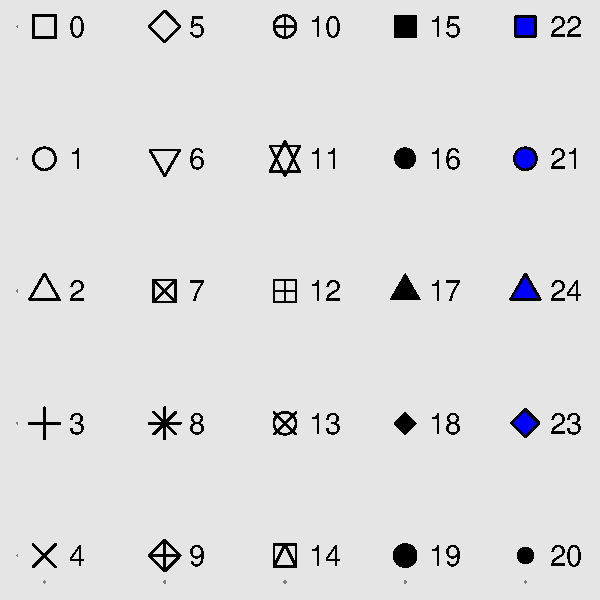
\includegraphics[width=0.45\linewidth]{diagrams/spec-shape}  
  }
  \subfigure[Horizontal and vertical justification settings.]{
    \label{fig:justification}
    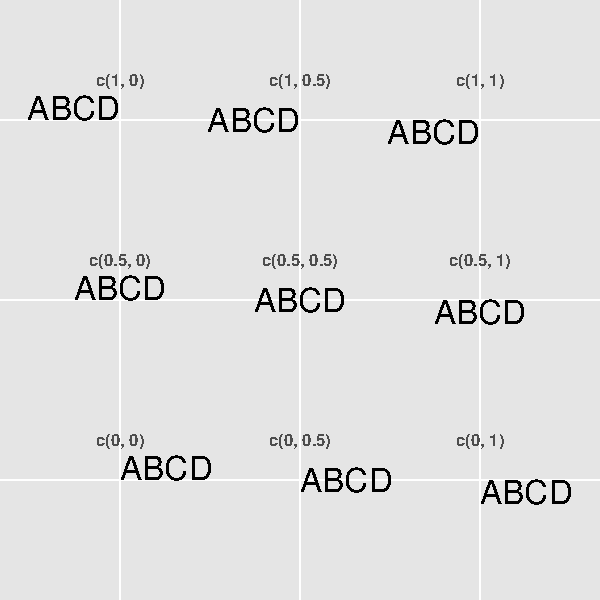
\includegraphics[width=0.45\linewidth]{diagrams/spec-justification}
  }
  \caption{Examples illustrating different aesthetic settings.}
\end{figure}
